\documentclass{mproj}
\usepackage{graphicx}

\usepackage{url}
\usepackage{fancyvrb}
\usepackage[final]{pdfpages}
\usepackage{times}

% for alternative page numbering use the following package
% and see documentation for commands
%\usepackage{fancyheadings}


% other potentially useful packages
%\uspackage{amssymb,amsmath}
%\usepackage{url}
%\usepackage{fancyvrb}
%\usepackage[final]{pdfpages}

\begin{document}

%%%%%%%%%%%%%%%%%%%%%%%%%%%%%%%%%%%%%%%%%%%%%%%%%%%%%%%%%%%%%%%%%%%
\title{Title of project placed here}
\author{Name of author placed here}
\date{Date of submission placed here}
\maketitle
%%%%%%%%%%%%%%%%%%%%%%%%%%%%%%%%%%%%%%%%%%%%%%%%%%%%%%%%%%%%%%%%%%%

%%%%%%%%%%%%%%%%%%%%%%%%%%%%%%%%%%%%%%%%%%%%%%%%%%%%%%%%%%%%%%%%%%%
\begin{abstract}
abstract goes here
\end{abstract}
%%%%%%%%%%%%%%%%%%%%%%%%%%%%%%%%%%%%%%%%%%%%%%%%%%%%%%%%%%%%%%%%%%%

%%%%%%%%%%%%%%%%%%%%%%%%%%%%%%%%%%%%%%%%%%%%%%%%%%%%%%%%%%%%%%%%%%%
\educationalconsent

%%%%%%%%%%%%%%%%%%%%%%%%%%%%%%%%%%%%%%%%%%%%%%%%%%%%%%%%%%%%%%%%%%%

\newpage
%%%%%%%%%%%%%%%%%%%%%%%%%%%%%%%%%%%%%%%%%%%%%%%%%%%%%%%%%%%%%%%%%%%
\section*{Acknowledgements}

acknowledgements go here sdfsdf

%%%%%%%%%%%%%%%%%%%%%%%%%%%%%%%%%%%%%%%%%%%%%%%%%%%%%%%%%%%%%%%%%%%
\tableofcontents
%%%%%%%%%%%%%%%%%%%%%%%%%%%%%%%%%%%%%%%%%%%%%%%%%%%%%%%%%%%%%%%%%%%

%%%%%%%%%%%%%%%%%%%%%%%%%%%%%%%%%%%%%%%%%%%%%%%%%%%%%%%%%%%%%%%%%%%
\chapter{Introduction}\label{intro}


I completed a program which allowed a turtlebot to autonomously map an environment using SLAM as well as create an inventory of items found in the environment.


\section{Importance/Context/Motivation}

Mobile robots are becoming more and more affordable and accessible which has allowed developers to take advantage of their applications in many different ways. 

SLAM has it's application in rescue robots which
http://www.aaai.org/Pressroom/Releases/release-02-0910.php
these robots required realtime control and utilised only video streams to identify and rescue people.

This compares to this which utilises rugged mobile robots to create SLAM maps of mine shafts with minimal supersvision. This can then be applied to areas which are too unsafe/ small for humans to access.
https://miningrox.informatik.tu-freiberg.de/en/

More affordable Drones can also be used to increasingly accurate create maps of property as well

Object detection can be used to detect humans via heat sensors etc. Aswell as identifying bombs etc.

\subsection{Sketch of how I achieved it}

\subsection{Objectives/Hypothesis Karl Popper/Problem statement}

\subsection{Description of Objectives}

\section{Outline of the dissertation}
%%%%%%%%%%%%%%%%%%%%%%%%%%%%%%%%%%%%%%%%%%%%%%%%%%%%%%%%%%%%%%%%%%%
\chapter{Background}\label{survey}

Existing/similar applications

Include Photos of everything
\section{Papers}
Semantic Slam
\section{Robot Operating System (ROS)}

ROS provides a meta-operating system to for robots to use which includes an abstraction of hardware, low level controllers, message passing and package management.
 
This means that ROS is generally independent of hardware specifics and has standard implementations in well known programming languages such as Python and C++.
 
Helps encourage code reuse through engineering principles of loose coupling which has helped provide a vibrant ecosystem of developers and researchers working on ROS applications.

ROS includes a powerful simulator in the form of Gazebo which allows whole applications to be written without use of a physical robot.

How ROS works?

Nodes are modular processes which can communicate with each other through messages which are data structures supporting typed fields such as primitives or arrays. These messages are transported via topics which can be subscribed or published to. 

\begin{figure}
  \caption{Illustration of the ROS concepts}
  \centering
  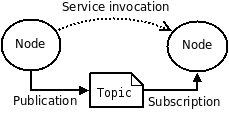
\includegraphics[width=0.5\textwidth]{images/ROS_basic_concepts.png}
  \label{fig:ROS diagram}
\end{figure}

For example one node can perform camera data processing while another one can control the robot's movement. These nodes can be publishing many messages to different topics, such as pointcloud messages to /camera/depth/points. The movement node can be subscribed to the /camera/depth/points topic and process it's messages. 



Coordinate transformation.
 
\section{Mobile Robots}
\subsection{Sensors}
\section{Turtlebot}
\section{Cameras}
\subsection{RGB-D}
\subsection{Stereo}
\section{SLAM}
\subsection{RtabMap}
\subsection{Others}
\section{Frontier Exploration}
\section{Object Detection}

At low levels of the evolutionary scale the eye acts as a type of goal detector rather than a camera. 

The information provided by past experience have a greater say on how a scene has been interpreted than immediate information provided by external organs.
The eye the brain the computer p208

However in contrast to simple organisms whose focus is on detection resulting in a sensitive and broad field of vision the programme must have the ability to classify which requires precise resolution when required.

Everything is seen for the first time.
Our sensory systems does not keep telling us things we already know as most important environmental information stays constant, this process is called adaption and happens not only at a retinal level but at higher levels in the brain.

What different types of neural structure are used to extract information from a visual signal

1) areas of high level of features
2) depth/closeness
3) shapes/edge detection - particularly light and dark

Not feasible to search for objects at all locations in a visual field
Partioning or perceptual organisation.

Law of proximity = Stimulus that are close together are percieved to be a group.

Geometric, Photometric modeling scene degmentation, naming+labeling,

Image matching:
correlation approach
 
feature matching approach
eges remain across two images of the same scene. 
relational matching approach

From page 281 --> talk about image labeling



\subsection{Feature Detection}
\subsection{Deep Learning}
\subsubsection{Tensorflow}
\subsubsection{Haar Cascades}
\subsubsection{Google Vision API}
\subsubsection{3D Detection}
\subsection{Summary}





%%%%%%%%%%%%%%%%%%%%%%%%%%%%%%%%%%%%%%%%%%%%%%%%%%%%%%%%%%%%%%%%%%%
\chapter{Approach/Implementation}
Describe what I did and How

What problems I encounted etc.

%%%%%%%%%%%%%%%%%%%%%%%%%%%%%%%%%%%%%%%%%%%%%%%%%%%%%%%%%%%%%%%%%%%
\chapter{System Design}

%%%%%%%%%%%%%%%%%%%%%%%%%%%%%%%%%%%%%%%%%%%%%%%%%%%%%%%%%%%%%%%%%%%
\chapter{System Implementation}
\section{Mapping}
\subsection{Transforming data}
\subsection{Calibration}
\section{Frontier Exploration}
\section{Object Detection and Recognition}
\subsection{Blob Detection}
\subsection{Detecting Clusters - different methods}
\subsection{Creating Boxes}
\subsection{Tracking Boxes}
\subsection{Positioning Boxes in Map/Loop Closure}
\subsection{Recognising Objects}
\subsection{Publishing to Rviz/Rtabmap}
\section{The whole package - how to utilise}
%%%%%%%%%%%%%%%%%%%%%%%%%%%%%%%%%%%%%%%%%%%%%%%%%%%%%%%%%%%%%%%%%%%
\chapter{Evaluation}
\section{Testing}

%%%%%%%%%%%%%%%%%%%%%%%%%%%%%%%%%%%%%%%%%%%%%%%%%%%%%%%%%%%%%%%%%%%
\chapter{Conclusion}\label{conclusion}
\subsection{Future work}

\appendix % first appendix
%%%%%%%%%%%%%%%%%%%%%%%%%%%%%%%%%%%%%%%%%%%%%%%%%%%%%%%%%%%%%%%%%%%
\chapter{First appendix}

\section{Section of first appendix}

%%%%%%%%%%%%%%%%%%%%%%%%%%%%%%%%%%%%%%%%%%%%%%%%%%%%%%%%%%%%%%%%%%%
\chapter{Second appendix}

%%%%%%%%%%%%%%%%%%%%%%%%%%%%%%%%%%%%%%%%%%%%%%%%%%%%%%%%%%%%%%%%%%%
% it is fine to change the bibliography style if you want
\bibliographystyle{plain}
\bibliography{mproj}
\end{document}
